\documentclass[11pt]{beamer}
\usetheme{PaloAlto}

\usepackage[utf8]{inputenc}
\usepackage[T1]{fontenc}
\usepackage{amsmath}
\usepackage{amsfonts}
\usepackage{amssymb}
\usepackage{forest}
\usepackage{url}

\setbeamercolor{logo}{bg=white}

\author{Christoph Teichmann \and Antoine Venant}
\title{The Dirichlet Categorial Model}

\subtitle{}

\logo{
\includegraphics[height=0.65cm]{SaarLogo}}

\institute{}

\date{}

\subject{}

\setbeamercovered{invisible}

\setbeamertemplate{navigation symbols}{}

\begin{document}
	
	\begin{frame}
		\maketitle
	\end{frame}
	
	\section{Goals}
	
	\begin{frame}{Teaching Goals}
		\begin{itemize}
			\item Basic properties of Dirichlet Distribution
			\item Dirichlet Categorial Model
			\item Chinese Restaurant Process
			\item How to build a simple language model from that
		\end{itemize}
	\end{frame}
	
	\section{Motivation}
	
	\begin{frame}{Categorial Variables in Computationl Linguistics}
		\centering
		We want probabilites for random variables with discrete outcomes:
				
		\begin{itemize}
			\item Next word given previous ones
			\item Children given parent in binary constituent tree
			\item Next Part-Of-Speech tag given previous ones
		\end{itemize}
		
		\vspace{20pt} Mary sees $\lbrace$ the, something, John, .\ $\rbrace$ \dots
	\end{frame}
	
	\begin{frame}{Categorial Variables in Computationl Linguistics}
		\centering
		We want probabilites for random variables with discrete outcomes:
		
		\begin{itemize}
			\item Next word given previous ones
			\item Children given parent in binary constituent tree
			\item Next Part-Of-Speech tag given previous ones
		\end{itemize}
		
		\begin{tabular}{lr}
			\begin{forest}
				[S [ NP [Mary] ] [VP [ sees ] [NP [\dots] ] ] ]
			\end{forest} &
			\begin{tabular}{c}
				$NP \rightarrow something$ \\
				$NP \rightarrow John$
			\end{tabular}
		\end{tabular}
	\end{frame}
	
	\section{A Simple Approach}
	
	\begin{frame}{The Next Word -- The Bayesian Approach}
		\centering
		\begin{itemize}
			\item<1-> Find a dataset relevant to your problem
			\begin{itemize}
				\item<2-> sentences from websites (tokenized) \checkmark
			\end{itemize}
			\item<1-> Reduce your problem to estimating a random quantity of interest
			\begin{itemize}
				\item<3-> Probabilities for next word in context \checkmark 
			\end{itemize}
			\item<1-> Build joint probabilistic model the data and the quantity to estimate
			\begin{itemize}
				\item<4-> uh oh
			\end{itemize}
		\end{itemize}
	\end{frame}
	
	\begin{frame}{Simple Model P(text|Probabilities)}
		\begin{itemize}
			\item N-Gram model
			\item $P_w(\text{w}_i|\text{w}_{i-1},\dots,\text{w}_{0}) = P_w(\text{w}_i|\text{w}_{i-1},\dots,\text{w}_{i-(n-1)})$
			\item let us start with $n=1$, i.e., Unigram Model: $P_w(\text{w}_i|\text{w}_{i-1},\dots,\text{w}_{0}) = P_w(\text{w}_i)$ 
		\end{itemize}
		
		\vspace{10pt}Model for data given word probabilities -- where to get word probabilities?
	\end{frame}
	
	\begin{frame}{Simplest Choice -- How to Write Word Probabilities}
		\begin{itemize}
			\item Assume finite lexicon $L$
			\item We will write the word probabilities as $P_w(x)$ for every $w \in L$
			\item $\left( \sum_{x \in L} P_w(x) \right) = 1$
			\item For all $x$ in $L$: $P_w(x) \geq 0$
			\item Write different distributions as $P_{w}^{x}$, $P_{w}^{y}$ \dots and $P_{w}^{X}$ as variable over probabilities
			\item Write prior, i.e.\ distribution over $P_{w}^{X}$ as $P_{\text{prior}}$
			\item Full joint model $P\left( P_{w}^{X},w_1,\dots,w_n \right)$
		\end{itemize}
	\end{frame}
	
	\begin{frame}{Simplest Choice -- Everything Equally Likely}
		\begin{itemize}
			\item Let us start with an uniform model, i.e.\ $P_{prior}\left( P^{x}_{w} \right) = \frac{1}{Z}$
			\item $Z$ is a constant to ensure integration to $1$
			\item We think $P^{x}_{w}(the) = 1$ is as likely as any other distribution
		\end{itemize}
		
		\vspace{10pt}Similar to model from last session
	\end{frame}
	
	\begin{frame}{How Does This Work}
		\begin{itemize}
			\item Lexicon: $L = \lbrace \text{Mary}, \text{sees}, \text{.}, \text{something}, \text{John}  \rbrace$
			\item Dataset: $D=$``Mary sees something''
			\item What is the Posterior, i.e., what is $P(P_{w}^X \vert w_3,w_2,w_1)$
			\item What is the next word? (hint: ``.'')
		\end{itemize}
	\end{frame}
	
	\begin{frame}{Posterior}
		\begin{align*}
			\overbrace{P(P_{w}^x \vert w_3,w_2,w_1)}^{\text{Posterior}} & \sim \left(\overbrace{\prod_{i \in \{1,2,3\}} P_{w}^{x}(w_i)}^{\text{Word Model}}\right) \overbrace{\frac{1}{Z}}^{\text{Prior}}
		\end{align*}
		
		\vspace{10pt} Is this (proportional to) a known distribution?
	\end{frame}
	
	\section{The Dirichlet Distribution}
	
	\begin{frame}{Is This A Known Distribution?}
		Dirichlet Distribution -- Distributions over probability distributions $P_X$ with outcomes $o_1,\dots,o_k$:
		
		\begin{align*}
			P_{Dir}(P_X) & = \frac{\prod_{i \in [1,K]} P_{X}(o_i)^{\alpha_i}}{B(\boldsymbol{\alpha})}
		\end{align*}
		
		\vspace{10pt} \begin{itemize}
			\item Here	$\alpha_i > 0$ are parameters -- there are lots of Dirichlet Distributions
			\item $B(\boldsymbol{\alpha})$ is a normalizer depending on all the $a_i$ -- look it up on Wikipedia
		\end{itemize}
	\end{frame}
	
	\begin{frame}{It is a Dirichlet Distribution!}
		\begin{align*}
			P_{Dir}(P_X) & = \frac{\prod_{i \in [1,K]} P_{X}(o_i)^{\alpha_i}}{B(\boldsymbol{\alpha})} \\
			P(P_{w}^x \vert w_3,w_2,w_1) & \sim \left(\prod_{i \in \{1,2,3\}} P_{w}^{x}(w_i)\right) \frac{1}{Z} \\
			& \sim \frac{\prod_{w' \in L} P_{w}^{x}(w')^{\sum_{i \in [1,3]} 1(w_i = w')}}{Z}
		\end{align*}
		
		\vspace{10pt}\begin{itemize}
			\item Here the $\alpha$s correspond to counts of how often we have seen each word $+1$
			\item Note that the uniform distribution over probability distributions is the same as the Dirichlet Distribution with $\boldsymbol{\alpha} = \boldsymbol{1}$ 
		\end{itemize}
	\end{frame}
	
	\begin{frame}{Visualizing a Dirichlet Distribution With Two Outcomes}
		\begin{center}
			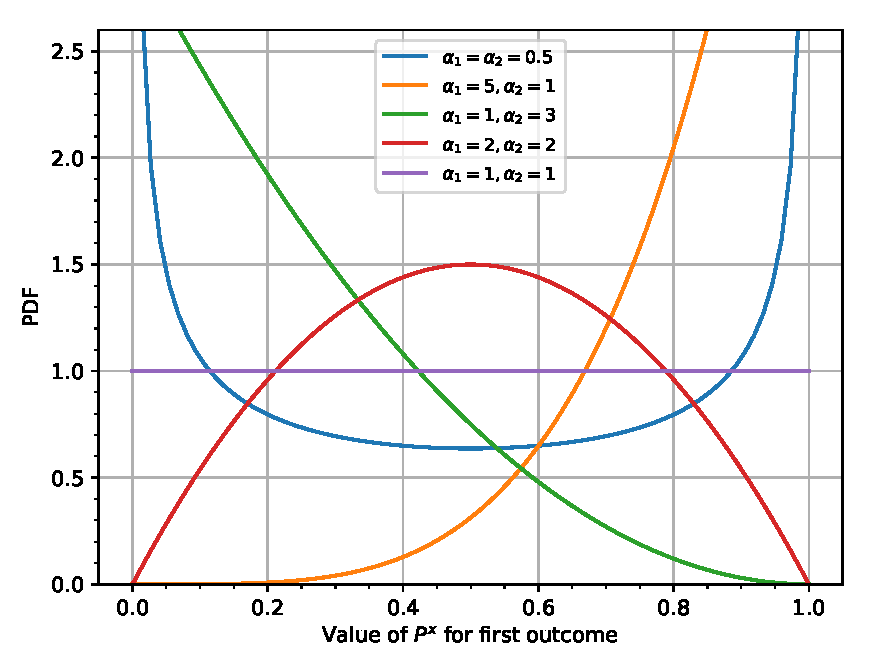
\includegraphics[width=0.75\linewidth]{dirichlet_distribution_pdf}
		\end{center}
		
		\begin{tiny}
			Generated with code based on code found at: \url{https://commons.wikimedia.org/wiki/File:Beta_distribution_pdf.svg} by user Horas based on the work of user Krishnavedala
		\end{tiny}
	\end{frame}
		
	\begin{frame}{Understanding the Behaviour of the Dirichlet}
		\begin{itemize}
			\item As all $\alpha$s concentrates at values proportional to $\alpha$s
			\item If all $\alpha$ are less than 1, then we favour ``sparse distributions'' few outcomes likely
		\end{itemize}
		
		\begin{tabular}{lr}
			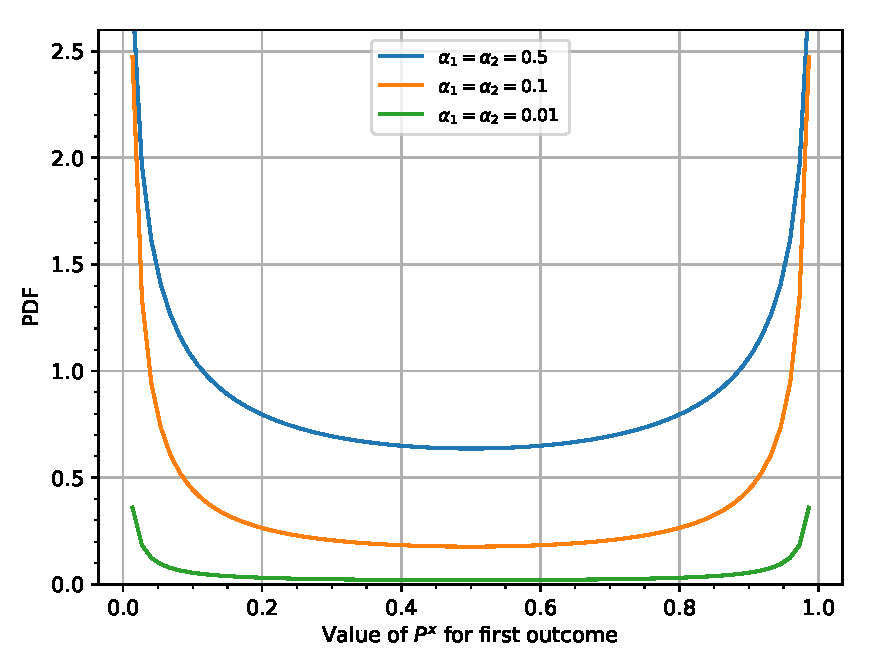
\includegraphics[width=0.49\linewidth]{dirichlet_distribution_sparse_pdf} &
			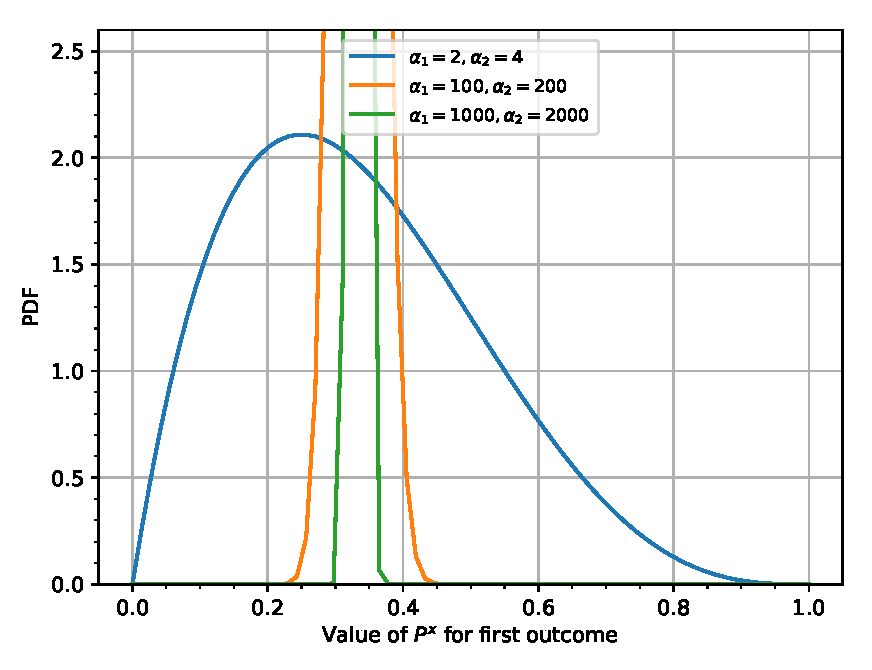
\includegraphics[width=0.49\linewidth]{dirichlet_distribution_dense_pdf} \\
		\end{tabular}
	\end{frame}
		
	\begin{frame}{Back to the Example}
		For our example our posterior is:

		\vspace{10pt}		
		\begin{align*}
			P(P_{w}^x) & = \left(\prod_{w_i \in L} P_{w}^{x}(w_i)^{\alpha_{w_i}}\right) \frac{1}{B(\boldsymbol{\alpha})}
		\end{align*}
	\end{frame}
	
	\section{Maximum Likelihood}
	
	\begin{frame}{Quick Diversion -- Maximum Likelihood}
		\begin{itemize}
			\item Lexicon: $L = \lbrace \text{Mary}, \text{sees}, \text{.}, \text{something}, \text{John}  \rbrace$
			\item Dataset: ``Mary sees something ?''
			\item What is the next word? (hint: ``.'')
		\end{itemize}
		
		WWMLD -- what would maximum likelihood do? - pick the model that makes the data most likely!
	\end{frame}
	
	\begin{frame}{Quick Diversion -- Maximum Likelihood}
		WWMLD --
		
		\begin{align*}
			P^{ml}_{w}(Mary) & = & \frac{1}{4}\\
			P^{ml}_{w}(sees) & = & \frac{1}{4}\\
			P^{ml}_{w}(something) & = & \frac{1}{4}\\
			P^{ml}_{w}(.) & = & 0 \\
			P^{ml}_{w}(John) & = & 0\\
		\end{align*}		
	\end{frame}
	
\end{document}